% White paper: downscaling 20CRv3 over India (build: make, in this directory)
\documentclass[11pt,a4paper]{article}

\usepackage[T1]{fontenc}
\usepackage[utf8]{inputenc}
\usepackage[sc]{mathpazo}
\usepackage[scaled=0.88]{helvet}
\usepackage[a4paper,margin=2.3cm]{geometry}
\usepackage{microtype}
\usepackage{graphicx}
\usepackage{booktabs}
\usepackage{tabularx}
\usepackage{threeparttable}
\usepackage[font=small,labelfont=bf,labelsep=period]{caption}
\usepackage{enumitem}
\usepackage[section]{placeins}  % floats stay in their section
\usepackage[round,authoryear]{natbib}
\usepackage{xcolor}
\usepackage[hidelinks]{hyperref}
\hypersetup{pdftitle={Downscaling the Twentieth Century Reanalysis over India},
  pdfauthor={Likith Muni Narakala}}

\graphicspath{{figures/}{../../results/figures/story/}}  % figures/ in the Overleaf package
\setlist{itemsep=2pt,topsep=4pt}
\setlength{\parskip}{3pt}

% ---- to fill in before release (shown in red until then) --------------------------------
\newcommand{\paperauthor}{Likith Muni Narakala}
\newcommand{\paperaffil}{\textcolor{red}{[affiliation]}}
\newcommand{\repourl}{\textcolor{red}{[GitHub URL]}}
\newcommand{\zenodo}{\textcolor{red}{[Zenodo DOI]}}
% ------------------------------------------------------------------------------------------

\newcommand{\twcr}{20CRv3}
\newcommand{\km}{\,km}
\newcommand{\mm}{\,mm}
\makeatletter\newcommand{\tablerows}[1]{\@@input #1 }\makeatother  % \input breaks \bottomrule

\title{\textbf{Downscaling the Twentieth Century Reanalysis over India}\\[4pt]
\large WRF and RegCM5 on the 1924 Kerala flood and the 26 July 2005 Mumbai cloudburst,\\
scored against criteria fixed in advance}
\author{\paperauthor\\[2pt]\small\paperaffil}
\date{White paper, October 2026}

\begin{document}
\maketitle

\begin{abstract}
\noindent Before 1940, atmospheric reanalyses rest on surface observations alone. The
NOAA--CIRES--DOE Twentieth Century Reanalysis version~3 (\twcr) assimilates only surface
pressure.
We test whether two regional climate models, WRF~4.5 and RegCM5, driven by \twcr\ at 12
and 3\km\ grid spacing, can reconstruct extreme west-coast monsoon rainfall over India.
Two events are simulated: the Kerala flood of July 1924 and the Mumbai cloudburst of
26 July 2005, the second also driven by ERA5 to separate driver error from model error.
Within each event all runs are scored on the same India Meteorological Department (IMD)
0.25$^\circ$ cells, against five criteria committed before any of the nine runs was started.
For 1924, downscaling turns the driver's weak, smooth rainfall (bias $-80$\%, pattern
correlation 0.51) into an orographic band along the Western Ghats (correlation 0.80--0.83
and bias $-39$\% at 12\km) and adds skill in all four runs, but the modelled rain peaks
three days after the observed peak.
For 2005, no model, resolution or driver reproduces the cloudburst: the largest 24\,h total
of any run within 50\km\ of Santacruz is 163\mm, against 944\mm\ observed.
The 3\km\ grids did not consistently improve on 12\km.
The spatial pattern of rainfall held in place by the terrain can be reconstructed from
\twcr, although too dry and too late; an organised convective extreme over the coastal plain
was not reproduced in this configuration. We also document an out-of-bounds table read in
the WRF Thompson microphysics that crashed every WRF run, and its fix. Code, namelists, scores and figures are public.
\end{abstract}

% ==========================================================================================
\section{Introduction}

Extreme rainfall events from before the satellite era are poorly known beyond the
station records that captured them. Reanalyses that assimilate upper-air observations
begin in the 1940s; ERA5 now reaches back to 1940. Earlier years are covered only by
reanalyses that assimilate surface observations alone: the Twentieth Century Reanalysis
\citep{compo2011}, ERA-20C \citep{poli2016} and the coupled CERA-20C
\citep{laloyaux2018}. We use the most recent of these, version~3 of the Twentieth Century
Reanalysis \citep[\twcr;][]{slivinski2019}, which assimilates only surface and sea-level
pressure observations, with prescribed sea-surface
temperature and sea ice, in an 80-member ensemble. Its circulation is therefore anchored by
observations, but its moisture and rainfall are products of the forecast model; its
performance is evaluated by \citet{slivinski2021}. On the 1$^\circ$ grid on which it is
distributed, the orography that shapes monsoon rainfall on the west coast of India is barely
resolved.

Dynamical downscaling can add that missing detail. WRF has been driven by the Twentieth
Century Reanalysis for three Vb cyclones over the Alps, of 2005, 1910 and 1876
\citep{stucki2020}, and by \twcr, with and without assimilation of early station
observations, for a cold-air outbreak in the 1816 ``year without a summer''
\citep{stucki2024}; 20CR has also been downscaled over China for present-day climate means
\citep{kong2015}. To our knowledge no study has downscaled \twcr\ for a South Asian monsoon
extreme, and none of the reanalysis downscaling studies above compares two regional models
on the same verification cells or fixes its success criteria before the simulations.

This white paper reports such an experiment. Two regional models, WRF \citep{skamarock2019}
and RegCM5 \citep{giorgi2023}, are run at 12\km\ (parameterised convection) and 3\km\
(convection-permitting) for one pre-1950 event, before ERA5 begins, and for one recent
event, when the same models can also be driven by ERA5
\citep{hersbach2020}. The recent event separates what the models can do from what the
historical driver allows. Five statements (H1--H5, Section~\ref{sec:verification}) were
committed to the repository before any of the nine runs was started, and all outcomes are
reported, failures included.

% ==========================================================================================
\section{Events}

\paragraph{E1: Kerala, July 1924.} The ``great flood of '99'' (Malayalam year 1099) followed
heavy monsoon rain over the Western Ghats of central Kerala; the Periyar basin counts it as
one of only two severe floods in its recent history \citep{sudheer2019}, and the 2018
floods were described as Kerala's worst since 1924 \citep{hunt2020}. A Central Water
Commission study describes the storm of 16--18 July 1924 over the High Ranges (Devikulam and
Munnar), with a three-day Kerala-average rainfall of 443\mm, more than the 414\mm\ of
15--17 August 2018 \citep{cwc2018}. ERA5 does not reach back to this event.

\paragraph{E2: Mumbai, 26 July 2005.} The Santacruz observatory recorded 944\mm\ in the
24\,h ending 08:30 IST on 27 July 2005, while Colaba in south Mumbai recorded 73\mm\
\citep{kumar2008}. In WRF simulations of the event, the Western Ghats and the land--sea
contrast together enhanced the rain by more than half, and an offshore mesoscale vortex
depended on latent heating \citep{kumar2008}. This event is driven by both \twcr\ and ERA5.

Both events are west-coast monsoon rainfall. Between them the era changes, and with it the
density of observations behind \twcr; so do the location and, as shown below, the
mechanism of the heaviest rain. Rainfall was chosen because IMD gridded
daily rainfall exists from 1901 \citep{pai2014}, so both eras can be verified on the same
grid.

% ==========================================================================================
\section{Models and set-up}

\begin{figure}[htbp]
  \centering
  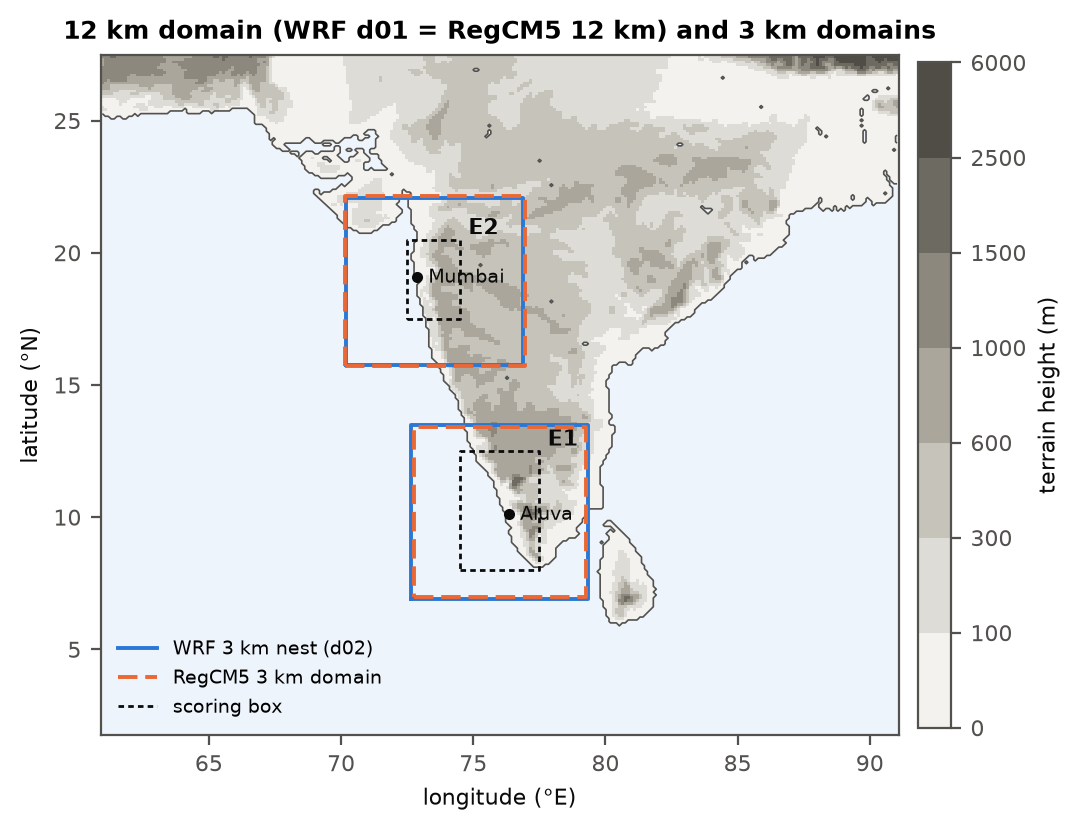
\includegraphics[width=0.66\textwidth]{fig1_domains.png}
  \caption{The shared 12\km\ domain (WRF d01 and the RegCM5 12\km\ grid) over terrain, the
  3\km\ domains of each model for each event (WRF blue, RegCM5 dashed orange) and the
  scoring boxes (black, finely dashed).}
  \label{fig:domains}
\end{figure}

Both models share one 12\km\ domain (271$\times$241 points, Mercator projection, 1.8--27.5$^\circ$N,
60.9--91.1$^\circ$E) and use a 3\km\ domain of 241$\times$241 points centred on each event's
scoring box (Fig.~\ref{fig:domains}). Each model runs in its reference configuration
(Table~\ref{tab:models}), so the comparison is between model systems rather than single
parameterisations. Neither model is nudged in the interior: the drivers act through the
initial state, the lateral boundaries and the sea-surface temperature. E1 runs from 00~UTC
12 July to 00~UTC 21 July 1924 (216\,h) and E2 from 00~UTC 24 July to 00~UTC 30 July 2005
(144\,h), each with 27\,h of spin-up before the first scored day.

\twcr\ is used as its ensemble mean (1$^\circ$, 28 pressure levels, 3-hourly) and ERA5 at
0.25$^\circ$ on 37 pressure levels, sub-sampled to 3-hourly. Both drivers pass through the
same code path in each model: Python writes WPS intermediate files for WRF and files in the
ERA5 layout of the RegCM5 pre-processor (which has no \twcr\ reader). The nine runs are
WRF (12 and 3\km\ in one run) and RegCM5 at 12 and 3\km\ for each of E1 with \twcr, E2 with
\twcr\ and E2 with ERA5; each driver's own rainfall is scored as the no-downscaling baseline.

\begin{table}[htbp]
\centering\small
\caption{Model configurations.}
\label{tab:models}
\begin{tabularx}{\textwidth}{@{}l>{\raggedright\arraybackslash}X>{\raggedright\arraybackslash}X@{}}
\toprule
 & WRF-ARW 4.5 & RegCM5 (MOLOCH non-hydrostatic core) \\
\midrule
Nesting & d01 12\km\ and d02 3\km\ in one run, one-way & 3\km\ run nested on the 12\km\ run's output \\
Levels, top & 50, 50\,hPa & 30 (12\km), 50 (3\km) \\
Time step & 60\,s / 15\,s & 90\,s / 30\,s \\
Microphysics & Thompson \citep{thompson2008}, with the bounds fix of Section~\ref{sec:thompson} & Nogherotto--Tompkins \citep{nogherotto2016} \\
Convection & Grell--Freitas \citep{grell2014} at 12\km, none at 3\km & Tiedtke \citep{tiedtke1989} at 12\km, none at 3\km \\
PBL & YSU \citep{hong2006} & Holtslag \\
Land surface & Noah, soil from the driver & BATS, RegCM5 default initial soil \\
Radiation & RRTMG \citep{iacono2008}, no aerosol & CCSM, no aerosol \\
SST & held at the initial value & updated from the driver every 3\,h \\
Lateral boundary & 5-point relaxation zone & exponential relaxation, 20 (12\km) / 31 (3\km) points \\
\bottomrule
\end{tabularx}
\end{table}

% ==========================================================================================
\section{Verification and criteria fixed in advance}
\label{sec:verification}

All rainfall is compared on the IMD 0.25$^\circ$ daily grid \citep{pai2014}, land cells only.
Model and driver rainfall are remapped onto it with an area-weighted (first-order
conservative) remap, so every run is scored on identical cells inside each event's scoring
box (Fig.~\ref{fig:domains}). Days are 24\,h windows ending at 03~UTC (08:30 IST, the IMD
observation time): seven days for E1 (13--20 July 1924) and four for E2 (25--29 July 2005).
The date convention of the IMD files was not assumed but read from the data: the 2005 box
maximum (732.5\mm) falls on the file's 27 July label, the morning on which the Santacruz
record was reported, so a label marks the end of its 24\,h window.

The metrics are the bias of the box-mean event total; the area-weighted pattern correlation
of event totals ($r$); the ratio of the largest daily cell value to the observed one (peak
ratio); the distance between the event-total maxima; the SAL structure, amplitude and
location components \citep{wernli2008}; and the fractions skill score
\citep[FSS;][]{roberts2008} pooled over the scored days at the IMD heavy, very heavy and
extremely heavy rainfall thresholds (64.5, 115.6 and 204.5\mm\,day$^{-1}$), here with a
5-point (1.25$^\circ$) neighbourhood unless stated. FSS is ``useful'' at or above
$0.5 + f_0/2$, with $f_0$ the observed fraction of cells above the threshold
\citep{roberts2008}. Added value (AV) is a run's score minus the score of its own driver's
rainfall on the same cells.

The five criteria below were committed to the repository on 15 October 2026 (UTC; commit
\texttt{260f8c9}, \texttt{docs/metrics.md}), before any of the nine runs was started, and
the file has not been changed since.
\begin{description}[leftmargin=2.2em,style=sameline,font=\normalfont\bfseries]
\item[H1] The models can produce E2 when the driver is good: with ERA5 at 3\km,
  FSS$_{115.6}$ at or above useful and $|$bias$|\le 30$\% for at least one model.
\item[H2] The historical driver costs little: for each model and resolution in E2, the
  FSS$_{115.6}$ with ERA5 exceeds that with \twcr\ by at most 0.15, and $|$bias$|\le 30$\%
  with \twcr.
\item[H3] Downscaling adds value: AV in FSS$_{64.5}$ is positive for every run.
\item[H4] 3\km\ beats 12\km\ on extremes: for each model and case, a peak ratio closer to 1
  and a higher FSS$_{115.6}$.
\item[H5] The pre-1950 event is reproduced: in E1 at 3\km, FSS$_{64.5}$ (9-point
  neighbourhood) at or above useful and $|$bias$|\le 40$\% for at least one model.
\end{description}

% ==========================================================================================
\section{Results}

\subsection{E1: the 1924 rain pattern rebuilt from surface pressure}

\begin{figure}[htbp]
  \centering
  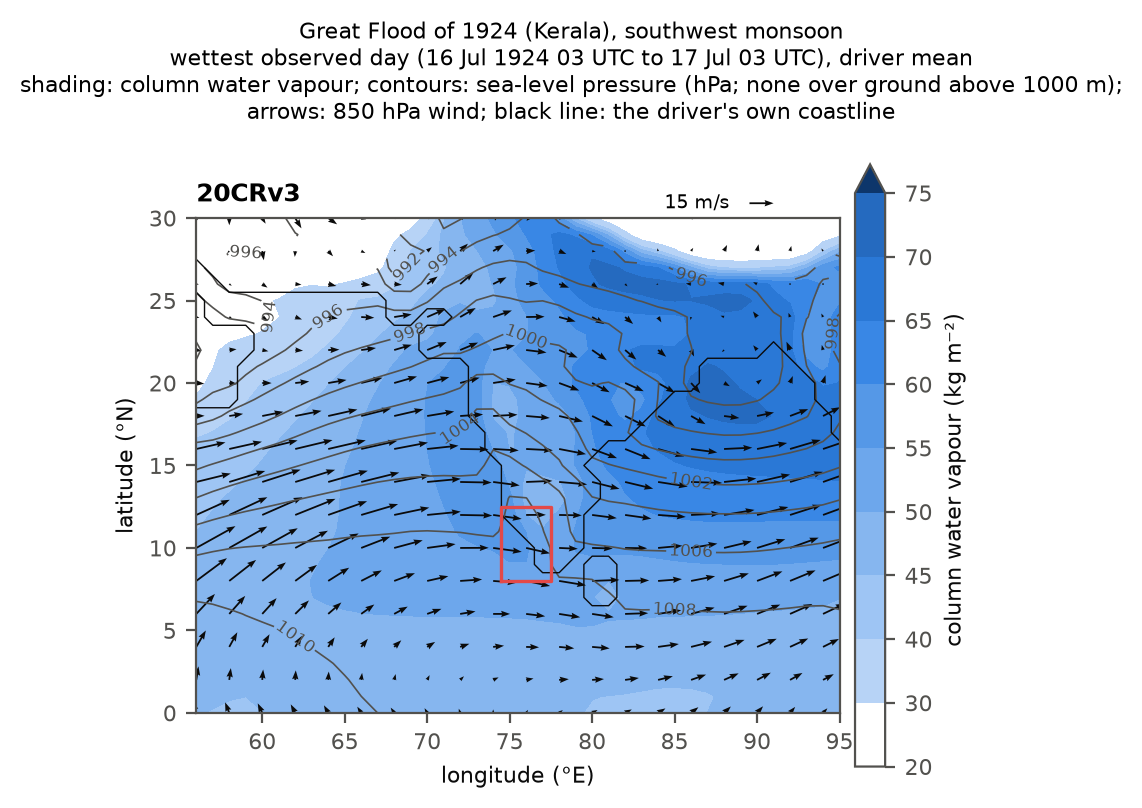
\includegraphics[width=0.56\textwidth]{fig2_E1_kerala1924_synoptic.png}
  \caption{\twcr\ ensemble mean on the wettest observed day of E1 (03~UTC 16 to 03~UTC
  17 July 1924): column water vapour (shading), sea-level pressure (contours, hPa) and
  850\,hPa wind (arrows). The red box is the scoring box; the black line is \twcr's own
  1$^\circ$ coastline.}
  \label{fig:e1syn}
\end{figure}

\begin{figure}[htbp]
  \centering
  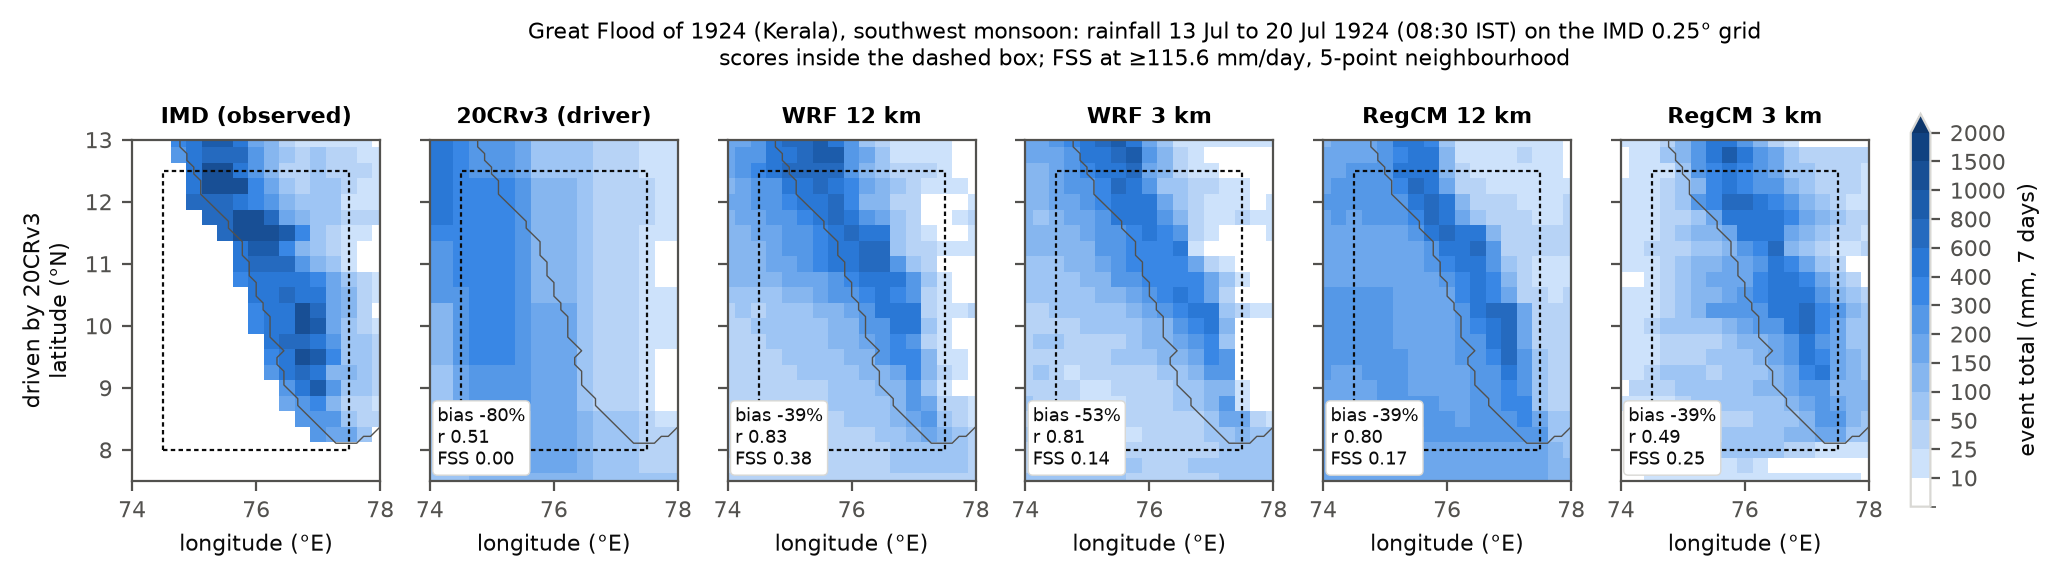
\includegraphics[width=\textwidth]{fig3_E1_kerala1924_totals.png}
  \caption{E1 rainfall, 13--20 July 1924, on the IMD grid: observed, the \twcr\ rainfall, and
  each downscaled run. Each panel gives its bias, pattern correlation and FSS at
  115.6\mm\,day$^{-1}$ inside the scoring box.}
  \label{fig:e1tot}
\end{figure}

\twcr\ holds the large-scale ingredients of an active monsoon spell on the wettest day:
a moist column over the Arabian Sea, strong 850\,hPa westerlies onto the Kerala coast and a
monsoon low near the head of the Bay of Bengal (Fig.~\ref{fig:e1syn}). Its own rainfall,
however, is a smooth field with no maximum on the Ghats: bias $-80$\%, pattern correlation
0.51, peak ratio 0.17, and no cell in the box above about 60\mm\,day$^{-1}$ on any day
(Figs.~\ref{fig:e1tot} and \ref{fig:e1day}, Table~\ref{tab:e1}).

Every downscaled run puts a band of heavy rain along the Western Ghats. At 12\km\ both
models reach a pattern correlation of 0.80--0.83 with a bias of $-39$\%; WRF places its
event-total maximum 27\km\ from the observed one. Peak ratios rise from 0.17 to 0.52--0.62,
and the added value in FSS$_{64.5}$ is $+0.58$ to $+0.71$ (H3 passes for all four runs).
The FSS at 204.5\mm\,day$^{-1}$ is zero for every run.

\begin{table}[htbp]
\centering\footnotesize
\caption{E1 scores, generated from the scoring output in \texttt{results/}. FSS with a
5-point neighbourhood; S, A, L are the SAL components.}
\label{tab:e1}
\begin{tabular}{@{}llrrrrrrrrr@{}}
\toprule
Run & Driver & Bias (\%) & $r$ & Peak & Max.\ dist.\ (km) & S & A & L & FSS$_{115.6}$ & FSS$_{204.5}$ \\
\multicolumn{2}{@{}l}{\emph{perfect}} & 0 & 1 & 1 & 0 & 0 & 0 & 0 & 1 & 1 \\
\midrule
\tablerows{tables/scores_E1_kerala1924.tex}
\bottomrule
\end{tabular}
\end{table}

\begin{figure}[htbp]
  \centering
  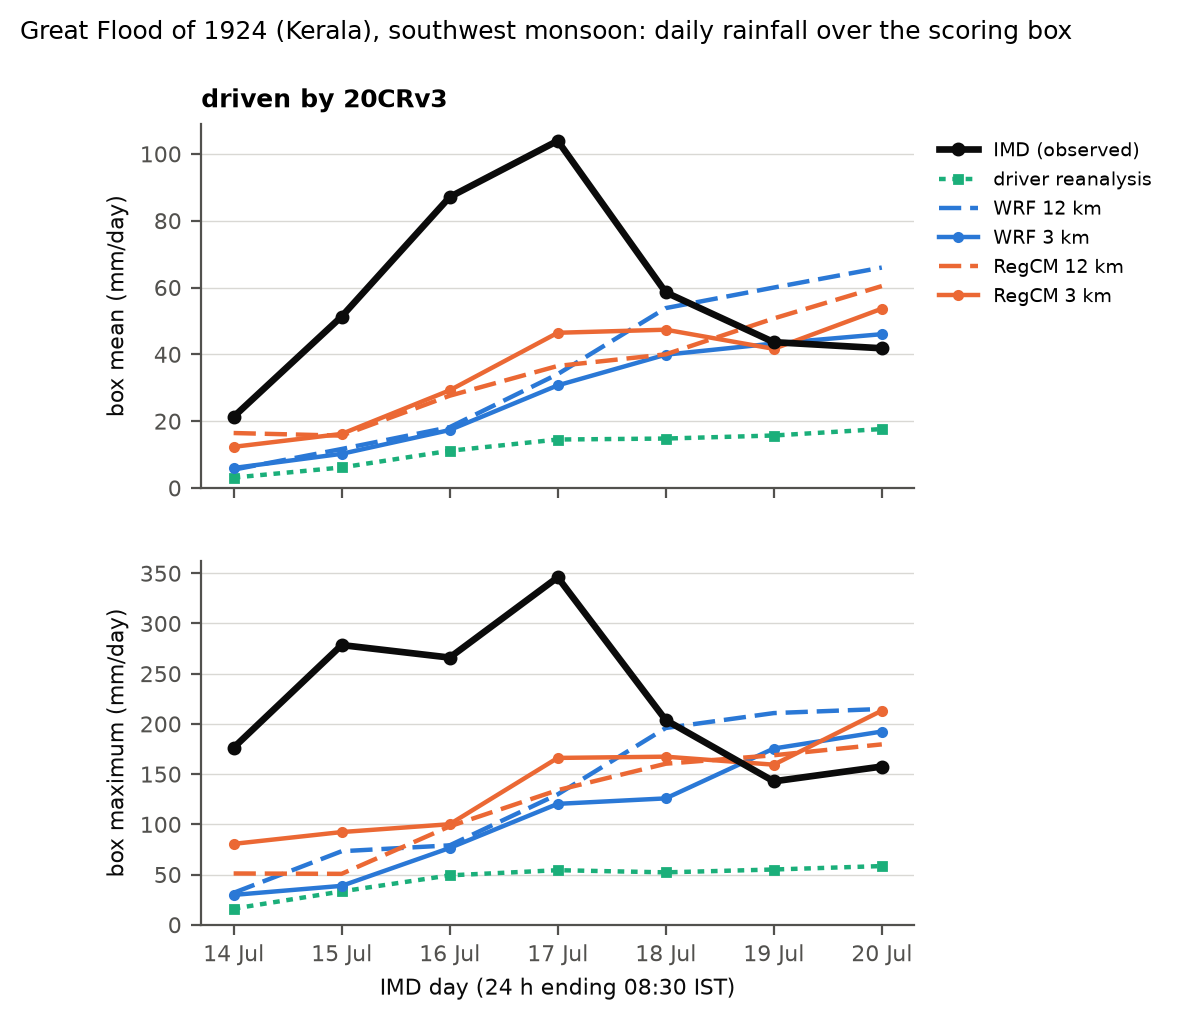
\includegraphics[width=0.58\textwidth]{fig5_E1_kerala1924_daily.png}
  \caption{E1 day by day over the scoring box: area mean (top) and largest cell value
  (bottom). IMD days end at 08:30 IST on the date shown.}
  \label{fig:e1day}
\end{figure}

The main shortcoming is timing (Fig.~\ref{fig:e1day}). The observed box mean rises to about
104\mm\ on IMD day 17 July, which matches the storm of 16--18 July, and falls afterwards.
Every downscaled run, and \twcr's own rainfall, has its wettest day on 20 July, the last
scored day and three days after the observed peak, when the observed box mean is below half
of its peak; their largest daily cell values reach 0.52--0.62 of the observed one. Because
the driver shows the same late build-up, the lag most likely enters
through the boundaries, from the timing of the monsoon surge in \twcr, rather than from
either regional model.

At 3\km, RegCM5 meets H5 by a narrow margin (FSS$_{64.5}$ with a 9-point neighbourhood
0.70 against a useful level of 0.68; bias $-39$\% against a limit of 40\%); WRF at 3\km\
does not (0.57; $-53$\%).

\subsection{E2: the cloudburst that no run produced}

\begin{figure}[htbp]
  \centering
  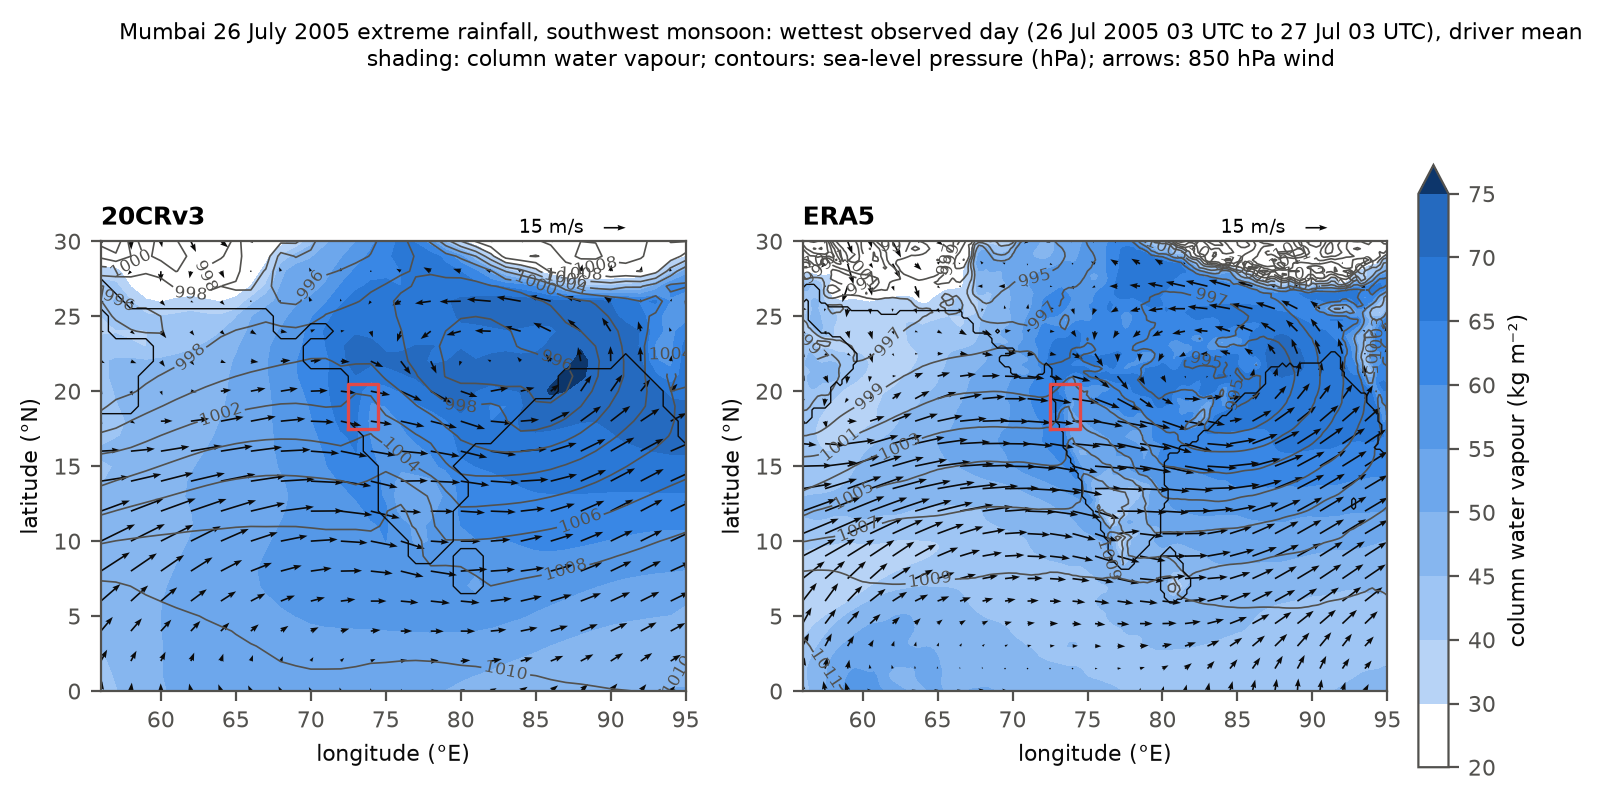
\includegraphics[width=\textwidth]{fig2_E2_mumbai2005_synoptic.png}
  \caption{As Fig.~\ref{fig:e1syn} for E2 (03~UTC 26 to 03~UTC 27 July 2005), \twcr\ (left)
  and ERA5 (right).}
  \label{fig:e2syn}
\end{figure}

\begin{figure}[htbp]
  \centering
  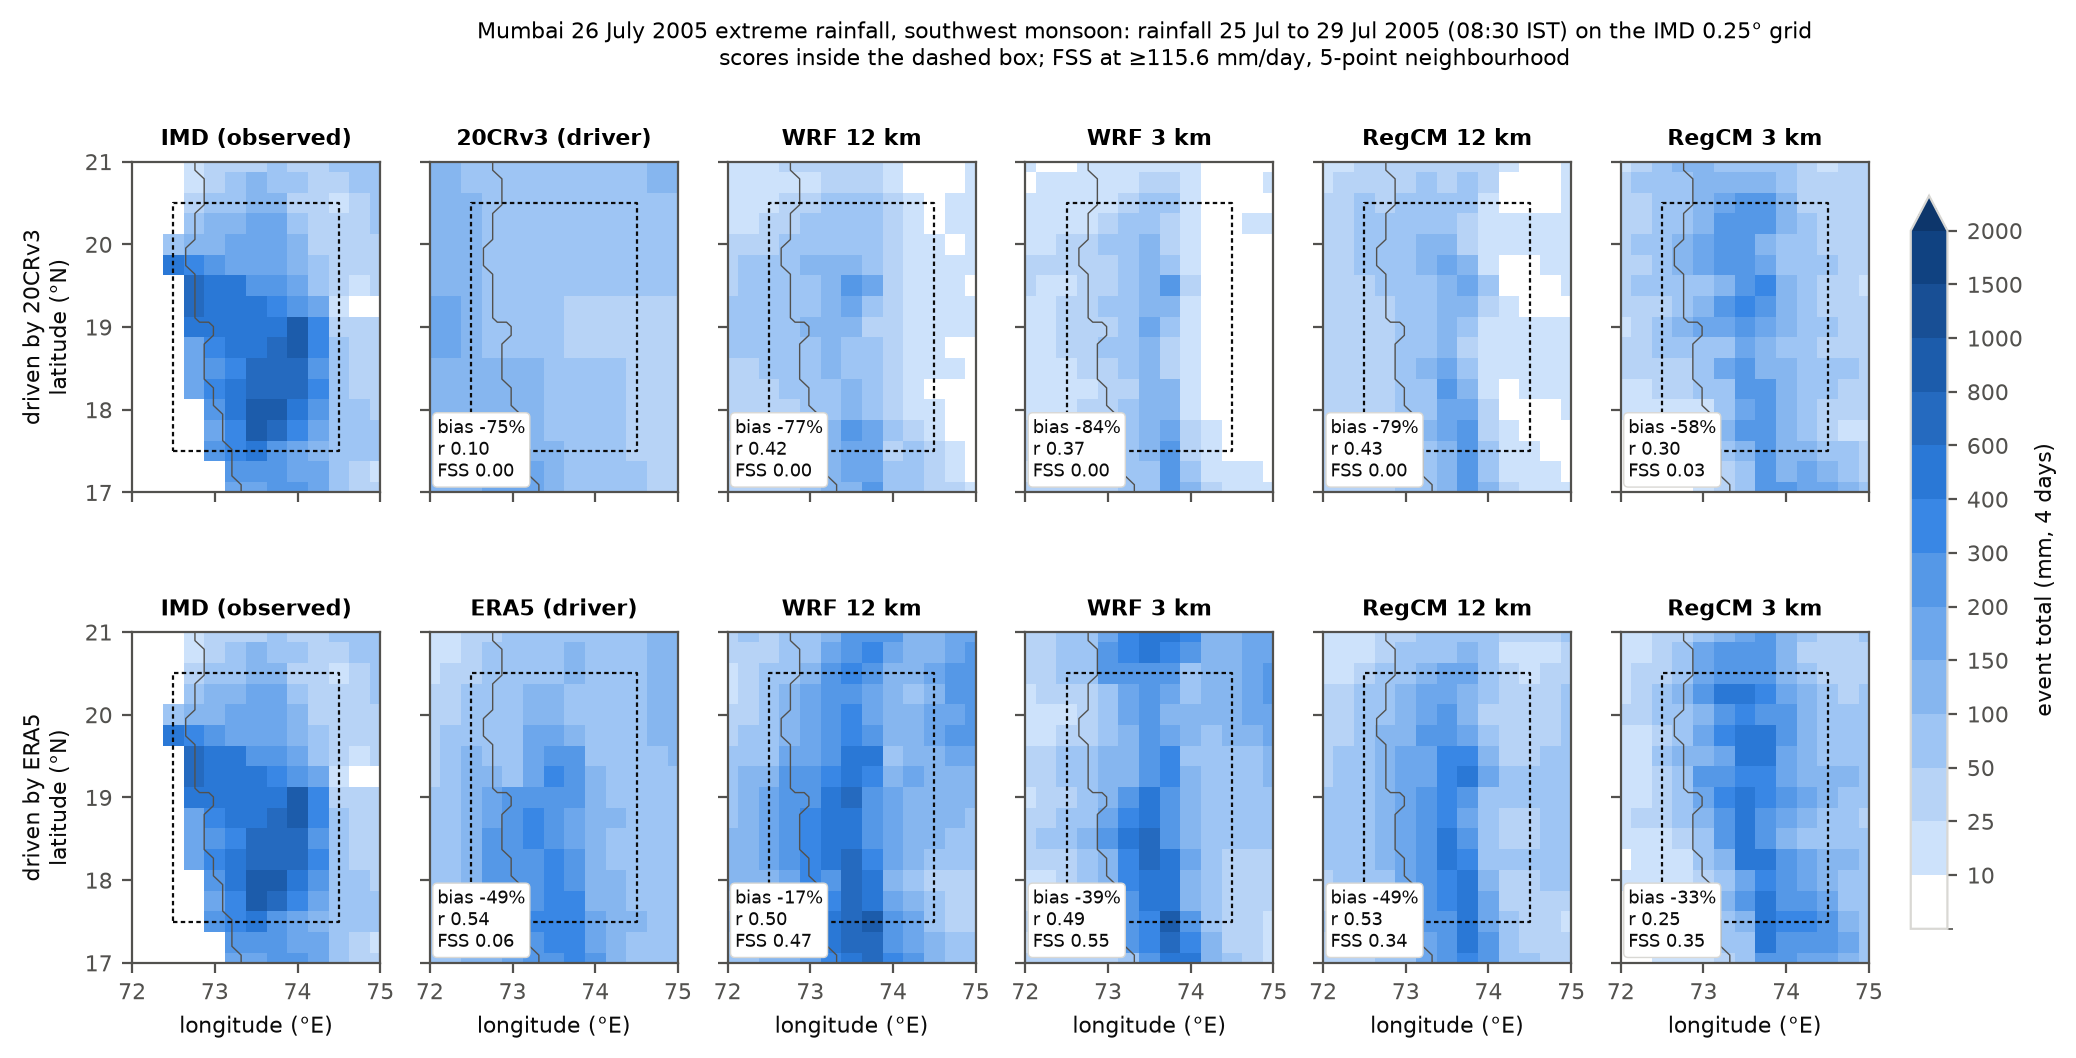
\includegraphics[width=\textwidth]{fig3_E2_mumbai2005_totals.png}
  \caption{As Fig.~\ref{fig:e1tot} for E2, 25--29 July 2005, driven by \twcr\ (top) and
  ERA5 (bottom).}
  \label{fig:e2tot}
\end{figure}

Both drivers place a monsoon low over central and eastern India with strong westerlies onto
the Konkan coast on 26 July (Fig.~\ref{fig:e2syn}); the large-scale setting for heavy rain
is present in both. The observed four-day rainfall covers the coastal plain and the Ghats
between about 17.5 and 19.5$^\circ$N, Mumbai included (Fig.~\ref{fig:e2tot}). The
ERA5-driven runs concentrate their rain in a narrow north--south band on the Ghats crest and
leave the coast with a fraction of the observed amount. They still give the best E2 scores:
WRF at 12\km\ has a bias of $-17$\%, and WRF at 3\km\ an FSS$_{115.6}$ of 0.55, just below the
useful level of 0.60 (Table~\ref{tab:e2}). Driven by \twcr, all four runs are 58--84\% too dry.

\begin{table}[htbp]
\centering\footnotesize
\caption{As Table~\ref{tab:e1} for E2.}
\label{tab:e2}
\begin{tabular}{@{}llrrrrrrrrr@{}}
\toprule
Run & Driver & Bias (\%) & $r$ & Peak & Max.\ dist.\ (km) & S & A & L & FSS$_{115.6}$ & FSS$_{204.5}$ \\
\multicolumn{2}{@{}l}{\emph{perfect}} & 0 & 1 & 1 & 0 & 0 & 0 & 0 & 1 & 1 \\
\midrule
\tablerows{tables/scores_E2_mumbai2005.tex}
\bottomrule
\end{tabular}
\end{table}

\begin{figure}[htbp]
  \centering
  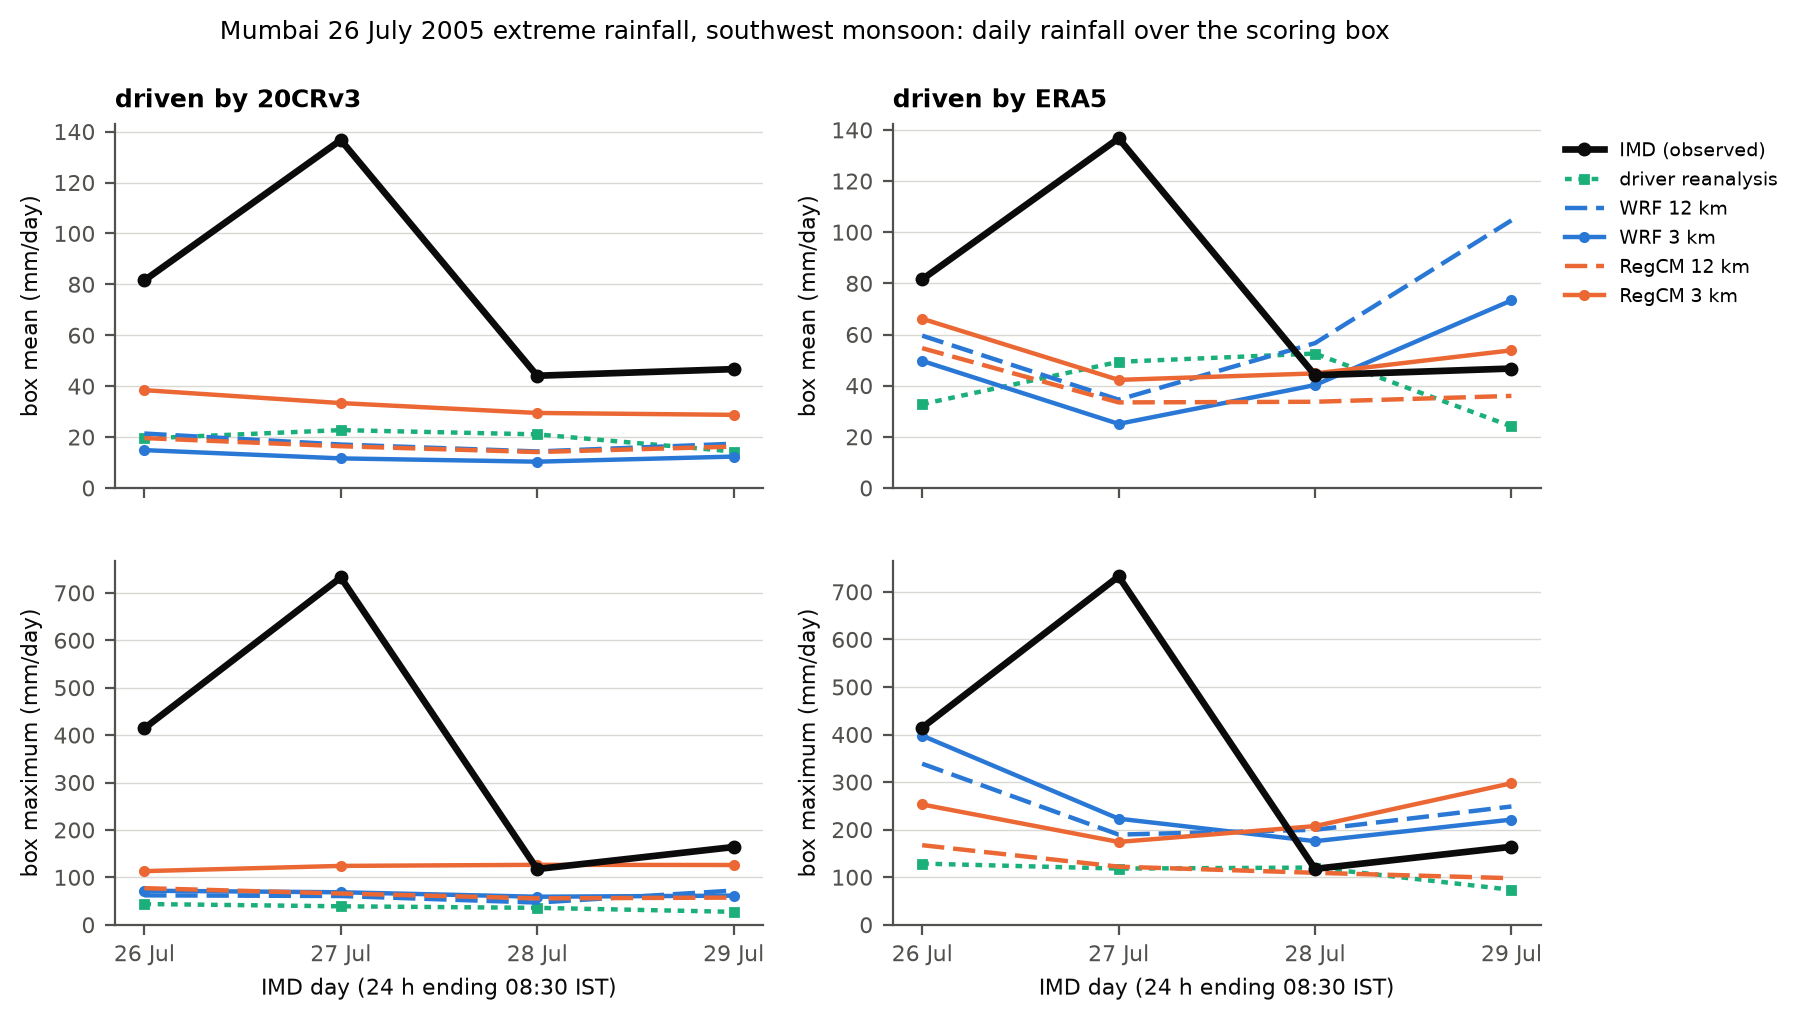
\includegraphics[width=\textwidth]{fig5_E2_mumbai2005_daily.png}
  \caption{As Fig.~\ref{fig:e1day} for E2, driven by \twcr\ (left) and ERA5 (right).}
  \label{fig:e2day}
\end{figure}

\begin{figure}[htbp]
  \centering
  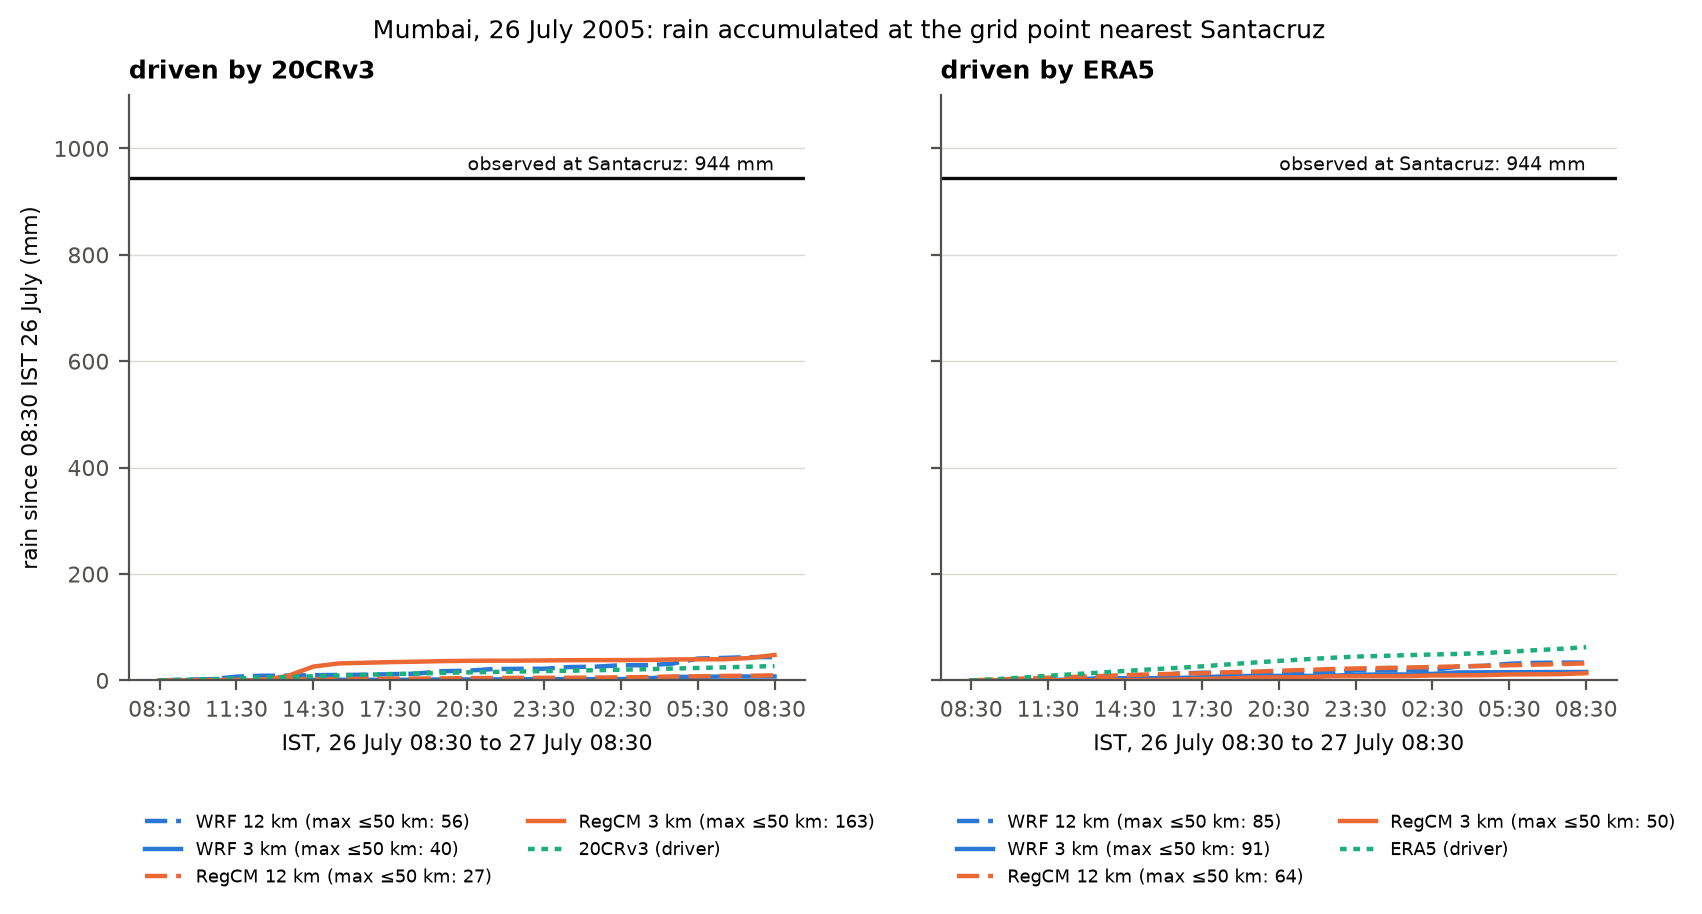
\includegraphics[width=\textwidth]{fig7_santacruz.png}
  \caption{Rain accumulated at the model grid point nearest the Santacruz observatory from
  08:30 IST 26 July to 08:30 IST 27 July 2005; the legend gives each run's largest 24\,h
  total within 50\km\ of Santacruz. The black line is the 944\mm\ observed.}
  \label{fig:scz}
\end{figure}

Day by day (Fig.~\ref{fig:e2day}), the ERA5-driven WRF runs come close to the observations
on the day before the event (WRF 3\km\ box maximum about 400\mm\ against about 415\mm). On the
cloudburst day, IMD day 27 July, the observed box mean jumps to about 137\mm\ and the box
maximum to 732.5\mm; every ERA5-driven run goes down instead, and the \twcr-driven runs stay
flat. At Santacruz itself (Fig.~\ref{fig:scz}), no run exceeds 100\mm\ in the 24\,h in which
944\mm\ was measured. The largest 24\,h total of any run within 50\km\ is 163\mm\ (RegCM5
3\km, \twcr); with ERA5 it is 91\mm\ (WRF 3\km).

H1 therefore fails: the best ERA5-driven 3\km\ run (WRF) reaches FSS$_{115.6}=0.55$ against
0.60, with a bias of $-39$\% against a limit of 30\%. H2 fails for every model and
resolution: replacing ERA5 by \twcr\ lowers FSS$_{115.6}$ by 0.31--0.55 and leaves biases of
$-58$ to $-84$\%. For H3, the \twcr-driven runs add value over their driver, but by only
$+0.01$ to $+0.05$ in three of the four (RegCM5 3\km: $+0.29$), while all four ERA5-driven
runs fall below ERA5's own FSS$_{64.5}$ of 0.70 ($-0.02$ to $-0.09$). At the higher
115.6\mm\ threshold, where ERA5 alone scores 0.06, the ERA5-driven runs score 0.34--0.55.

\subsection{Does 3\,km help?}

\begin{figure}[htbp]
  \centering
  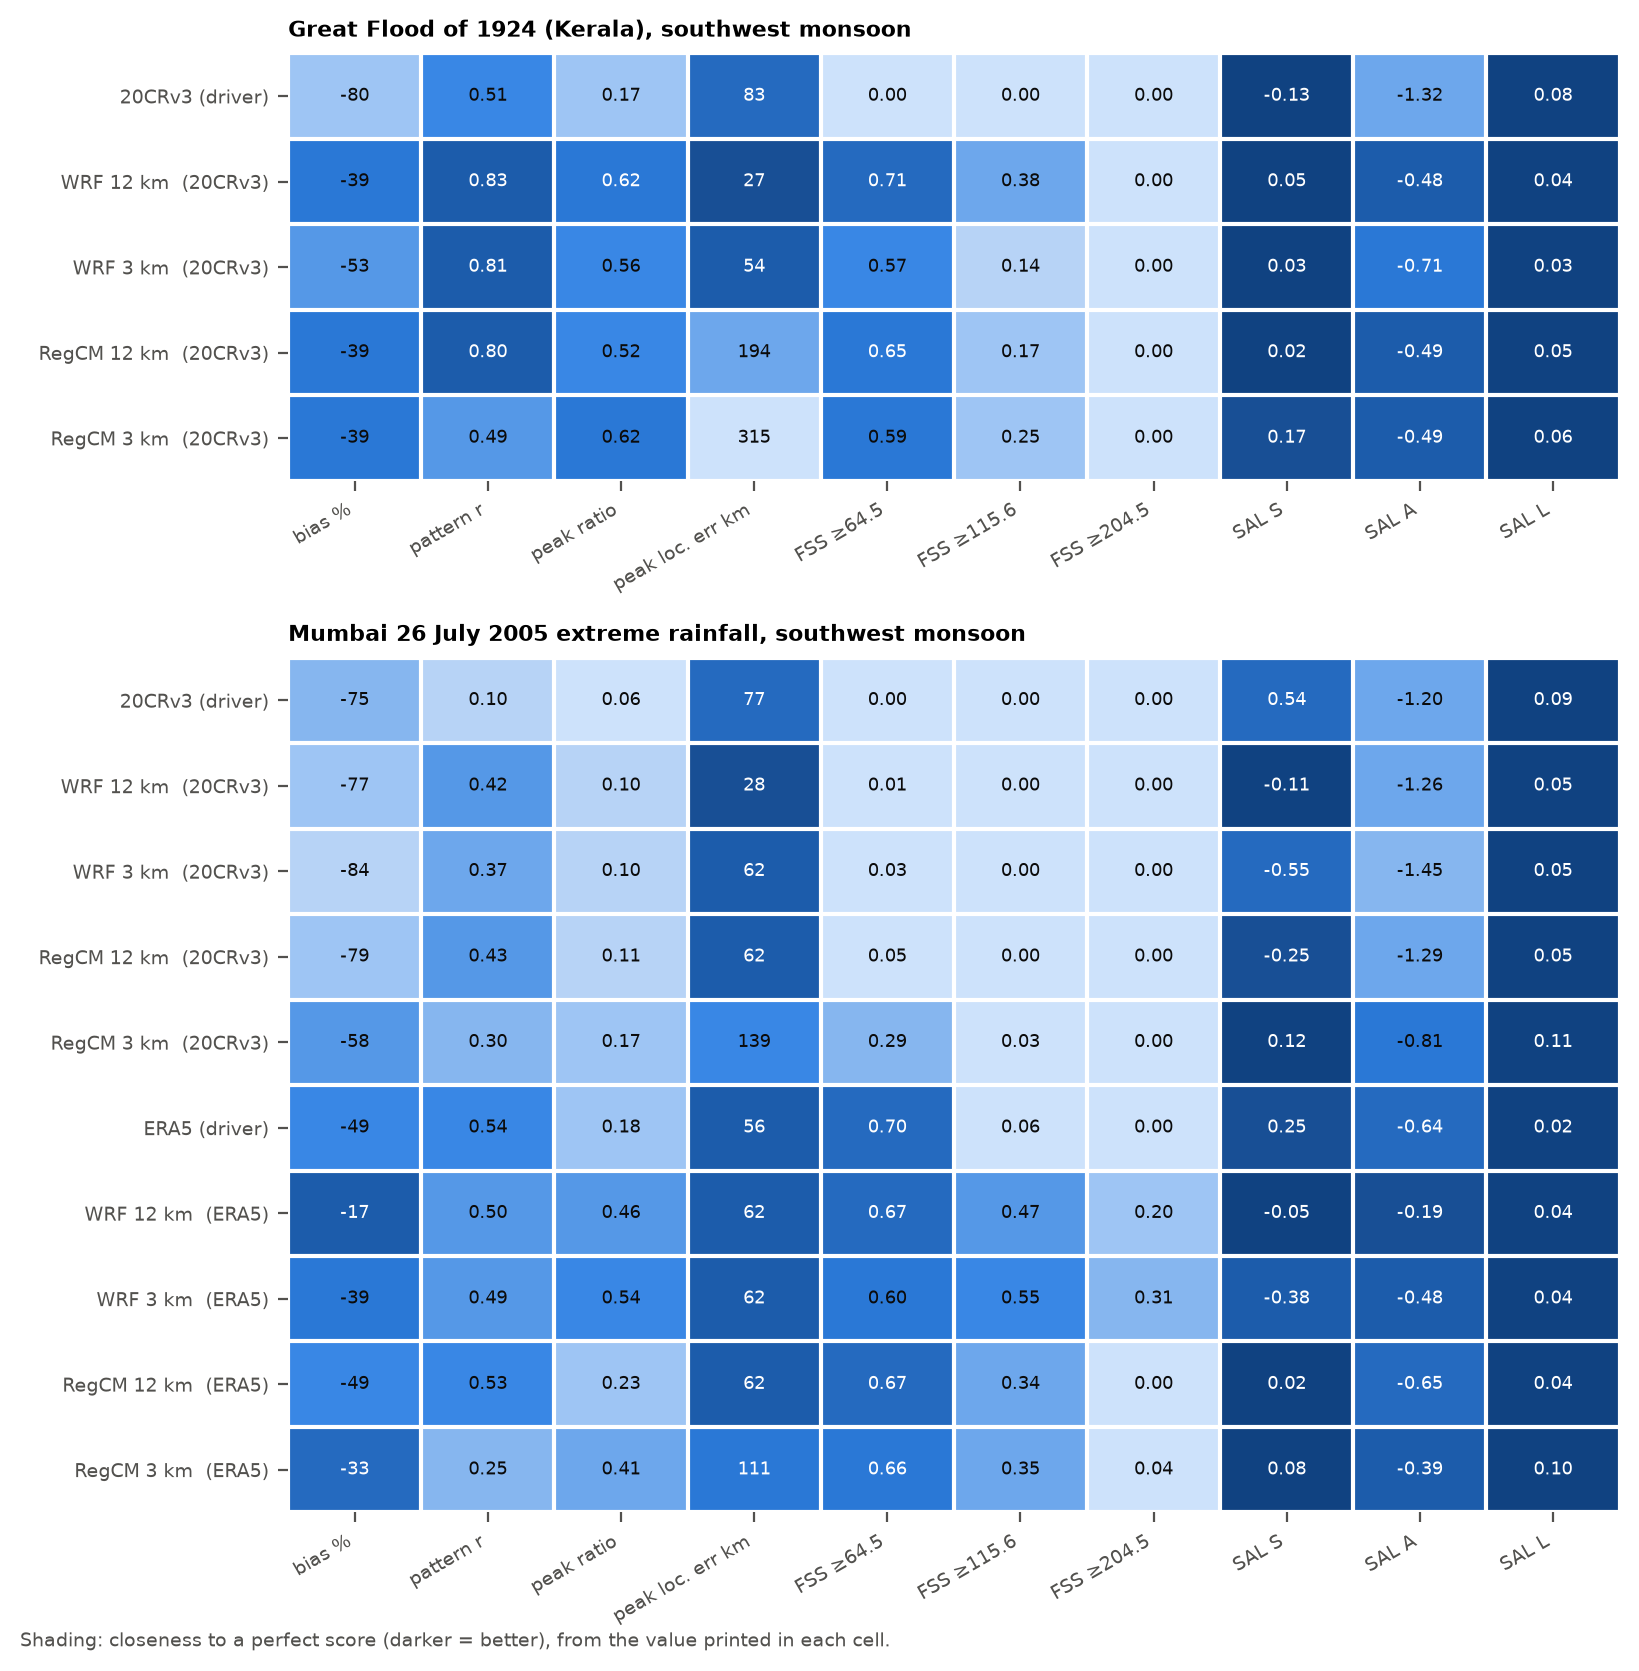
\includegraphics[width=0.95\textwidth]{fig6_scores.png}
  \caption{All headline scores. Shading shows closeness to a perfect score (darker is better),
  computed from the value printed in each cell.}
  \label{fig:scores}
\end{figure}

H4 passes in four of six cases (Fig.~\ref{fig:scores}). WRF at 3\km, with no cumulus scheme,
is drier than WRF at 12\km\ with Grell--Freitas in every case: E1 $-39$ to $-53$\%, E2 with
\twcr\ $-77$ to $-84$\%, E2 with ERA5 $-17$ to $-39$\%. With ERA5 it still sharpens the
extremes (peak ratio 0.46 to 0.54, FSS$_{115.6}$ 0.47 to 0.55), but with \twcr\ in 1924 it
loses them (FSS$_{115.6}$ 0.38 to 0.14). RegCM5 at 3\km\ is as wet as or wetter than at
12\km\ and raises the peak ratio in all three cases (E1 0.52 to 0.62; E2 \twcr\ 0.11 to
0.17; E2 ERA5 0.23 to 0.41), but its pattern correlation drops (E1 0.80 to 0.49; E2 ERA5
0.53 to 0.25) and its event-total maximum lies 111--315\km\ from the observed one
(native 3\km\ fields in Fig.~\ref{fig:native}).

% ==========================================================================================
\section{Discussion}

\paragraph{Terrain-held rain versus organised convection.} The contrast between the two
events is the main result. In 1924, the heaviest rain lay along the Ghats, where the
lifting is set by the terrain; a regional model given roughly the right onshore flow puts
rain in the right place, even from a 1$^\circ$ reanalysis that assimilates only pressure.
In 2005, the extreme came from organised convection over the coastal plain, which depends
on mesoscale details that neither driver supplies directly and that the models did not
generate. The ERA5-driven runs placed their rain on the Ghats crest, as for 1924, and
missed the coastal maximum.

\paragraph{What the driver sets.} The late build-up in 1924 is shared by \twcr's own
rainfall and every downscaled run, so the regional models inherited it. The 2005 synoptic
setting is similar in both drivers (Fig.~\ref{fig:e2syn}), yet the \twcr-driven runs are
far drier than the ERA5-driven ones (H2). The difference most likely lies in what the
regional models receive from the driver (initial state, lateral boundaries or sea-surface
temperature), for example the strength and moisture of the low-level flow; we have not
diagnosed it. Ensemble
members of \twcr, rather than its mean, would show how much of either error is chance.

\paragraph{Added value depends on the driver and the threshold.} Over a 1$^\circ$ driver
without orographic rain, every run adds value. Over ERA5, which already scores FSS 0.70 at
64.5\mm, downscaling lowers the FSS at that threshold by 0.02--0.09 but adds $+0.28$ to
$+0.49$ at 115.6\mm, consistent with the view that a regional model can add value mainly at scales the
driver does not resolve \citep{diluca2012}.

\paragraph{Resolution and physics.} Convection-permitting grids are expected to improve
heavy, short-duration rainfall \citep{prein2015}; with two cases and daily totals we see
mixed results, and WRF without a cumulus scheme rained less than WRF with one in every case.
The 2005 event is known to be sensitive to the physics: with WRF from the same start time,
\citet{kumar2008}, with the Grell--Dévényi cumulus scheme \citep{grell2002} on their 33 and
11\km\ domains, WSM6 microphysics and an explicit 3.6\km\ nest, captured the Santacruz
rainfall; with Kain--Fritsch or Betts--Miller--Janjić on the outer domains the rain was
underestimated by more than half. Our WRF
configuration (Thompson and Grell--Freitas) is one that misses it; whether the physics alone
explains the miss was not tested here.

% ==========================================================================================
\section{Technical findings}

\subsection{An out-of-bounds read in WRF Thompson microphysics}
\label{sec:thompson}

All three WRF runs first stopped with segmentation faults in the Thompson
microphysics (\texttt{mp\_physics\,=\,8}): E1 after 117.6 simulated hours, E2 with \twcr\ after 74\,h and
E2 with ERA5 after 8.3\,h, with no CFL warnings and ample memory. All three faulted at the
same machine instruction. In WRF 4.5, when hail-aware graupel is off, the rain--graupel
collection tables are allocated with a graupel-density dimension of extent 1, but the eight
lookups into them use a graupel-density index of 5. Each lookup therefore reads the wrong
table entry, and in the heaviest rain with graupel it reads beyond the end of the table.
A one-column test of WRF 4.5's own module with Fortran bounds checking stops at one of these
lookups. The same lookups are unchanged in WRF 4.5.1 to 4.7.1. Our fix clamps the
index to the table extent (\texttt{MIN(idx\_bg(k),}\linebreak[0]\,\texttt{dimNRHG)}), which leaves the hail-aware
scheme (\texttt{mp\_physics\,=\,38}) unchanged, and adds the two Thompson changes of WRF 4.5.1.
With it, all three runs completed from the initial time without a single stop. The patch and
the one-column reproducer are in the repository.

\subsection{Reading the observation date convention from the data}

The first scoring run used an assumed IMD date convention that turned out to be wrong by
one day, comparing every model day with the following observed day. A check that reads the
convention from the 2005 record (Section~\ref{sec:verification}) caught it; the first
scorecard was discarded, and the scoring code now refuses to run when the check fails.

\subsection{Cost}

The nine runs used 1{,}891 core-hours, two-thirds of them for WRF, against a planning
estimate of 741--1{,}482, on a shared node with more processes than cores. WRF took
28--30\,h of wall time per run on 12--20 cores; RegCM5 took 1.4--3.2\,h at 12\km\ and
5.9--13.2\,h at 3\km\ on 20 cores.

% ==========================================================================================
\section{Limitations}

Two events are case studies, and the criteria are pass/fail statements per case, without
significance testing. Each event is one deterministic run from the \twcr\ ensemble mean.
H5 passes by 0.02 in FSS and 0.6 percentage points of bias. Other century-long
reanalyses (ERA-20C, CERA-20C) were not tried as drivers. The 1924 IMD grid rests on fewer
gauges than the 2005 grid. Present-day land use is used for 1924, and the two models
initialise soil moisture differently. The Santacruz figure is a station total, compared
with grid-point and 50\km\ values.

\section{Outlook}

\begin{itemize}
\item \textbf{Ensembles of the driver.} Downscaling a set of \twcr\ members would give a
  distribution of rainfall against which an observed extreme can be judged, and separate
  driver uncertainty from chance in convection.
\item \textbf{Physics as part of the ensemble.} Starting with the Grell--Dévényi and WSM6
  combination of \citet{kumar2008} in this set-up.
\item \textbf{Bias correction} of the downscaled pre-1950 rainfall ($-39$\% in three of four
  E1 runs), tested on further IMD-era monsoon extremes before 1950.
\end{itemize}

\section*{Code and data availability}

Code, configuration, namelists, scores and figures: \repourl; archived version: \zenodo.
\twcr\ is available from NOAA PSL, ERA5 from the Copernicus Climate Change Service, and the
IMD gridded rainfall from the India Meteorological Department.

\section*{Acknowledgements}

Support for the Twentieth Century Reanalysis Project version 3 dataset is provided by the
U.S. Department of Energy, Office of Science Biological and Environmental Research (BER), by
the National Oceanic and Atmospheric Administration Climate Program Office, and by the NOAA
Physical Sciences Laboratory. ERA5 is produced by the Copernicus Climate Change Service at
ECMWF. Rainfall observations are from the India Meteorological Department. WRF is developed
by NCAR and RegCM5 by ICTP.

\bibliographystyle{abbrvnat}
\bibliography{refs}

% ==========================================================================================
\appendix
\section{All criteria outcomes}

\begin{center}\footnotesize
\begin{tabular}{@{}llll@{}}
\toprule
ID & Case & Values & Result \\
\midrule
\tablerows{tables/hypotheses.tex}
\bottomrule
\end{tabular}
\end{center}

\clearpage
\section{Event totals on the 3\,km grids}

\begin{figure}[h]
  \centering
  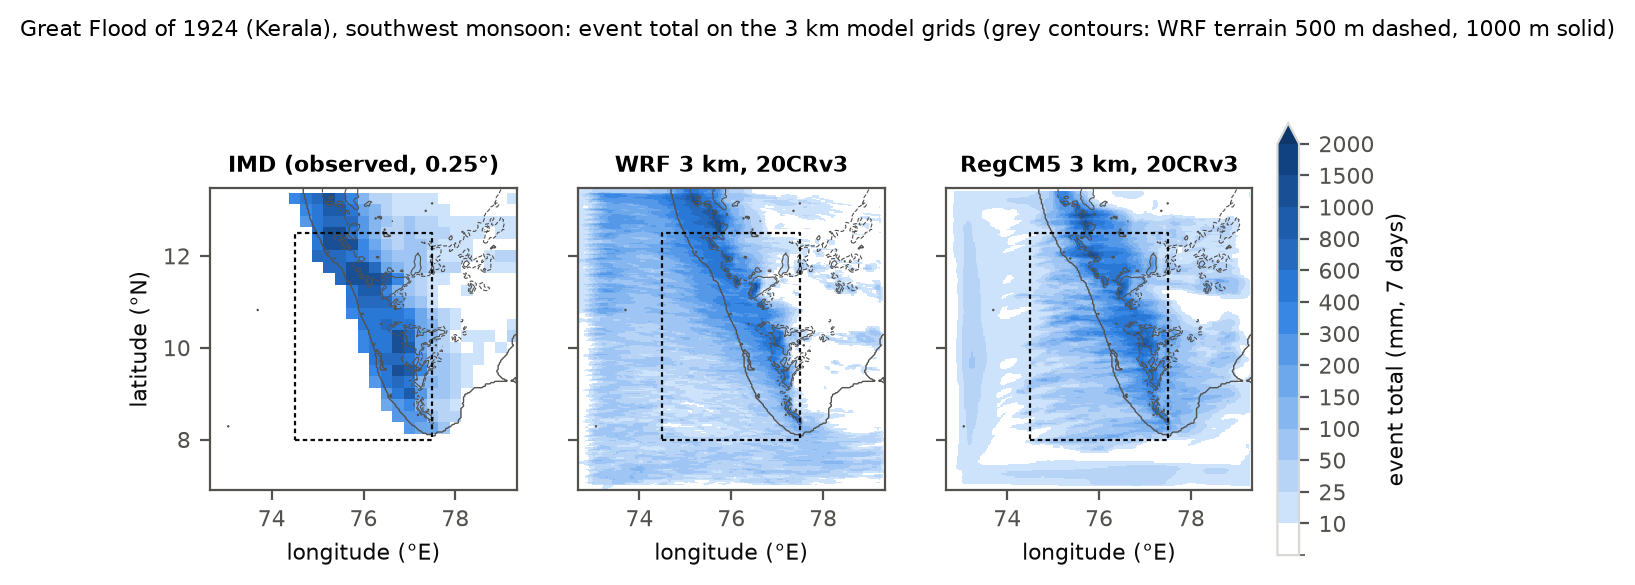
\includegraphics[width=\textwidth]{fig4_E1_kerala1924_native.png}\\[4pt]
  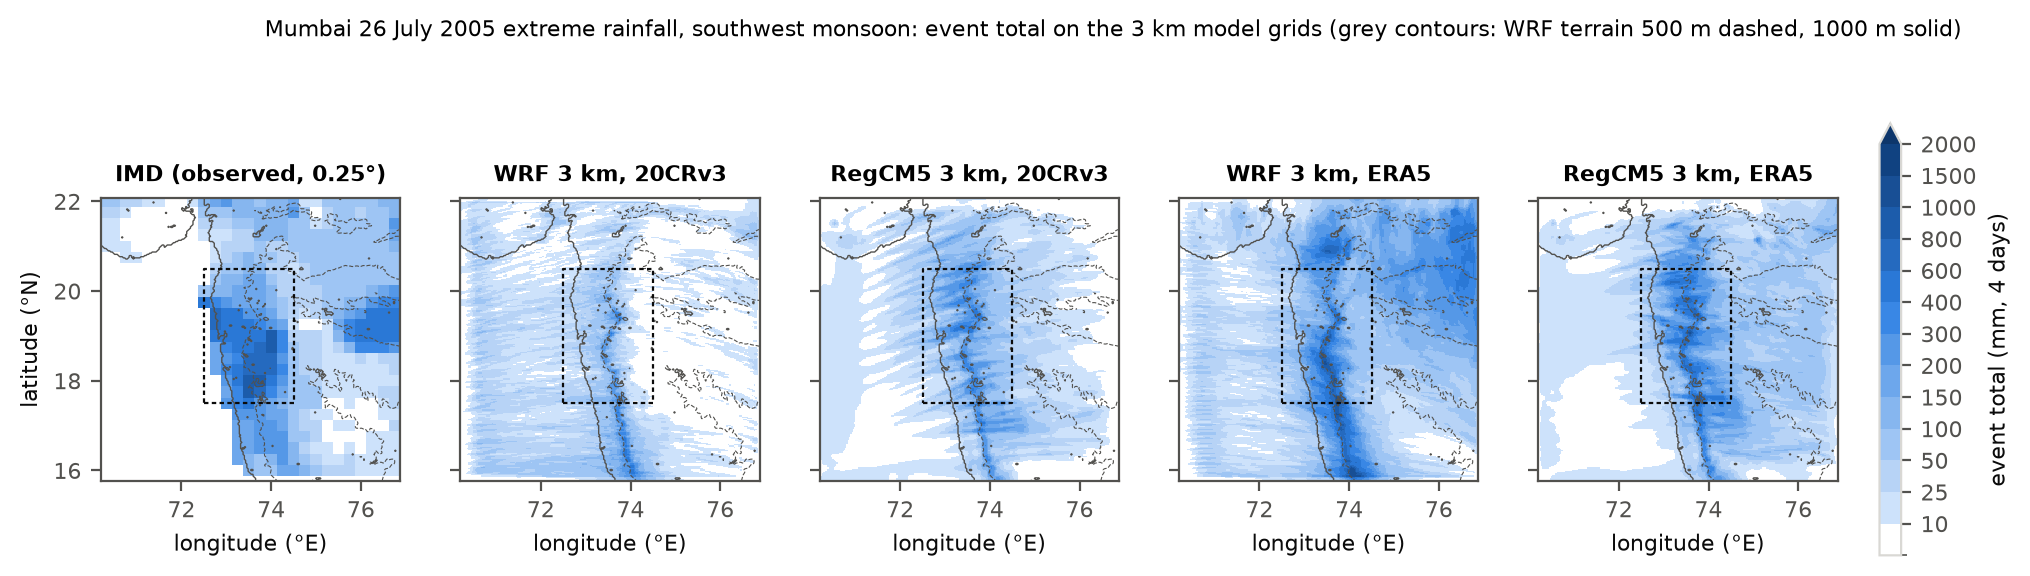
\includegraphics[width=\textwidth]{fig4_E2_mumbai2005_native.png}
  \caption{Event totals on the native 3\km\ grids with WRF terrain contours, E1 (top) and E2
  (bottom). The east--west streaks over the sea lie along the low-level westerlies; the pale
  frame around the RegCM5 domain is its lateral relaxation zone. Neither affects the scores,
  which use IMD land cells only.}
  \label{fig:native}
\end{figure}

\end{document}
